%Przykładowy plik ułatwiający złożenie projektu dyplomowego inżynierskiego.
%UWAGA: Generowany napis na stronie tytułowej o treści PROJEKT DYPLOMOWY INŻYNIERSKI został zaproponowany przeze mnie i nie jest, póki co, potwierdzony przez władze wydziału. Przed ostatecznym oddaniem tak złożonej pracy należy upewnić się jaka powinna być treść tego napisu. W momencie gdy uzyskam informację na temat treści tego napisu, dokonam niezbędnych zmian w źródłach.

\documentclass[en,printmode]{mgr}
%opcje klasy dokumentu mgr.cls zostały opisane w dołączonej instrukcji

%poniżej deklaracje użycia pakietów, usunąć to co jest niepotrzebne
%\usepackage{polski} %przydatne podczas składania dokumentów w j. polskim
\usepackage[utf8]{inputenc}
\usepackage[T1]{fontenc} %poprawne składanie polskich czcionek
%pakiety do grafiki
\usepackage{graphicx}
\usepackage{subcaption}
\usepackage{psfrag}

%pakiety dodające dużo dodatkowych poleceń matematycznych
\usepackage{amsmath}
\usepackage{amsfonts}

%pakiety wspomagające i poprawiające składanie tabel
\usepackage{supertabular}
\usepackage{array}
\usepackage{tabularx}
\usepackage{hhline}
\usepackage{multirow}
\usepackage{indentfirst}
\usepackage{enumitem}

\usepackage{breqn}

\newcommand{\floor}[1]{\left\lfloor #1 \right\rfloor}
\usepackage[justification=centering]{caption}

%pakiet wypisujący na marginesie etykiety równań i rysunków zdefiniowanych przez \label{}, chcąc wygenerować finalną wersję dokumentu wystarczy usunąć poniższą linię
%\usepackage{showlabels}


%definicje własnych poleceń
\newcommand{\R}{I\!\!R} %symbol liczb rzeczywistych, działa tylko w trybie matematycznym
\newtheorem{theorem}{Twierdzenie}[section] %nowe otoczenie do składania twierdzeń

%dane do złożenia strony tytułowej
\title{System lokalizacji samolotów z wykorzystaniem ADS-B}
\engtitle{Airplane tracking system using ADS-B}
\author{Karol Szpila}
\supervisor{\vfil Ph.D., D.Sc. Grzegorz Budzyń\\
\\ Institute of Telecommunications, Teleinformatics and Acoustics (I-28)}
%\guardian{dr hab. inż. Imię Nazwisko Prof. PWr, I-6} %nie używać jeśli opiekun jest tą samą osobą co prowadzący pracę

%\date{2008} %standardowo u dołu strony tytułowej umieszczany jest bieżący rok, to polecenie pozwala wstawić dowolny rok

%poniżej jest lista kierunków i specjalności na wydziale elektroniki, należy wybrać właściwe lub dopisać jeśli nie ma odpowiednich
\field{Elektronika (EKA)}
\specialisation{Advanced Applied Electronics(AAE)}
%\specialisation{Robotyka (ARR)}
%\specialisation{Komputerowe sieci sterowania (ARK)}
%\specialisation{Systemy informatyczne w automatyce (ASI)}
%\specialisation{Komputerowe systemy zarządzania \\procesami produkcyjnymi (ARS)}
%\field{Elektronika i telekomunikacja (EIT)}
%\specialisation{Akustyka (ETA)}
%\specialisation{Aparatura elektroniczna (EAE)}
%\specialisation{Elektroniczne i komputerowe \\systemy automatyki (ESA)}
%\specialisation{Zastosowania inżynierii komputerowej \\w technice (EZI)}
%\specialisation{Inżynieria dźwięku (EID)}
%\specialisation{Elektronika stosowana \\i optokomunikacja (TEO)}
%\specialisation{Telekomunikacyjne sieci szerokopasmowe (TSS)}
%\specialisation{Teleinformatyczne sieci mobilne (TSM)}
%\specialisation{Sygnały w telekomunikacji cyfrowej (TSC)}
%\specialisation{Teleinformatyczne systemy rozsiewcze (TSR)}
%\field{Informatyka (INF)}
%\specialisation{Systemy informatyki w medycynie \\i technice (IMT)}
%\specialisation{Inżynieria systemów informatycznych (INS)}
%\specialisation{Inżynieria internetowa (INT)}
%\specialisation{Systemy i sieci komputerowe (ISK)}
%\field{Teleinformatyka (TIN)}
%\specialisation{Teleinformatyka (TIN)}

%tutaj zaczyna się właściwa treść dokumentu
\begin{document}
%\bibliographystyle{plabbrv} %tylko gdy używamy BibTeXa, ustawia polski styl bibliografii

\maketitle %polecenie generujące stronę tytułową
%\dedication{6cm}{To jest przykładowa treść opcjonalnej dedykacji, należy ją zmienić lub usunąć w całości polecenie \texttt{$\backslash$dedication}}

\chapter*{Nomenclature}
\begin{table}[!htb]
\begin{tabular}{ll}
$ADC$  & Analog to Digital Converter   \\
$DAC$  & Digital to Analog Converter   \\
$FPGA$ & Field Programmable Gate Array \\
$SDR$  & Software Defined Radio \\
$QAM$  & Quadrature Amplitude Modulation \\
$RF$   & Radio Frequency \\
$SoC$  & System on Chip   \\
$SPI$  &

$UART$                        
\end{tabular}
\end{table}

\tableofcontents %spis treści

%poniżej znajduje się przykładowa treść dalszej części dokumentu, zainteresowanych zachęcam do rozszyfrowania frazy "Lorem ipsum" :)
\let\cleardoublepage\clearpage %usuwa puste strony pomiaedzy rozdziałami

\chapter{Introduction}
	\section{Purpose and aim}
			The purpose of this paper is to study various parameters defining RF signal quality and models of IQ
		imbalance. Research concept of Software Defined Radio, principles of operation of such devices and capability
		of Xilinx Zynq SoC in such domain. Evaluate different correction algorithms implementation. Compare it
		performance for various type of signals: singletone, multitone, broadband, and 4-QAM, 8-QAM8 and 16-QAM
		modulated. The comparison include simulation in Matlab, implementation hardware (FPGA part of ZYNQ SoC) and 			native correction inside RF transceiver chip.
		
	\section{Thesis outline}
	
\chapter{Theoretical background}
	In this chapter the theoretical operation of quadrature modulators and demodulators is explained. Widely
		used in RF communication IQ signal model is explained together with it imbalance model. For last the
	Software Defined Radio concept is presented.
	\section{Theoretical operation quadrature modulator/demodulator}
		
	\section{IQ signal model}
			The term IQ is an abbreviation for in-phase and quadrature. Signal are considered in-phase when phase
		of both is equal and quadrature when it differs by 90$\deg$. IQ data model shows changes in phase and
		magnitude of a sine wave. Modification of these parameters allow to encode information upon a sine wave.
		\\
		
		\noindent				
		Equation of the sine wave is:
		\[
			A cos\left(2\pi f t+ \phi\right), \label{eq:sinewave}
		\]
		where:
		\begin{itemize}
			\item $A$ is amplitude,
			\item $f$ is frequency,
			\item $\phi$ is phase shift
		\end{itemize}
		
		According to equation \label{eq:sinewave} only amplitude, phase and frequency of the sine wave can be
		modified. Moreover frequency is first derivative of phase. Therefore it can be collectively referred to 
		as the phase angle. According to these assumptions the instantaneous state of a sine wave can be described
		in complex plain using magnitude and phase as polar coordinates.
		
		\begin{figure}[!htb]
    		\centering
   			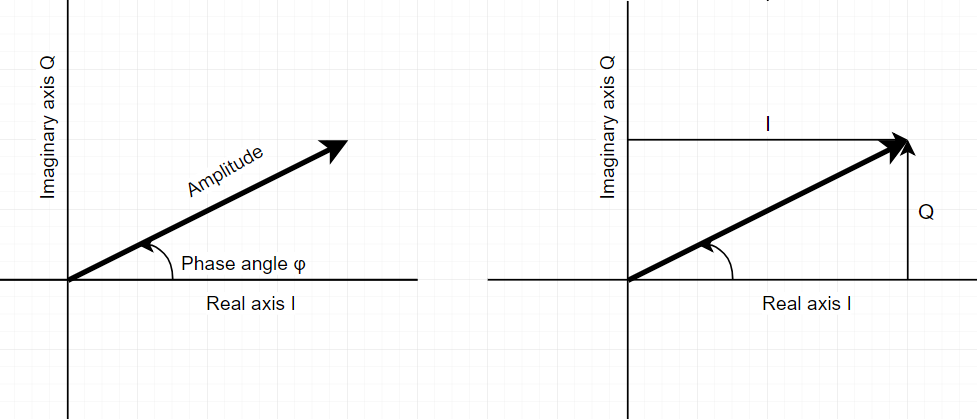
\includegraphics[width=\textwidth]{plots/polarplots.png}
    		\caption{\textit{Representation of sine wave in complex plain}}
    		\label{fig:polarplot}
		\end{figure}
		
		\newpage
		Using trigonometry, the polar coordinates can be converted into I and Q components of the signal using
		equations:
		\begin{itemize}
			\item $I = A cos\left(2\pi f t\right)$, \label{eq:IQ}
			\item $Q = A sin\left(2\pi f t\right)$,
		\end{itemize}
		
		IQ data model is widely used in RF communication systems. It allows to distinguish type of modulation used 
		on carrier. Allows to introduce concept of positive and negative frequency. Amplitude and phase angle form
		seems to be more intuitive, however precisely varying the phase of a high-frequency carrier sine wave in a
		hardware circuit according to an input message signal is difficult. Therefore such hardware modulators will
		be expensive and hard to design and build. To avoid direct modulation of RF signal phase signal is decomposed
		to I and Q components.
		\\
		
		According to Ptolemy’s identitie for the cosine of sum:
		\[
			cos\left(x+y\right) = 
			cos\left(x\right)  cos\left(y\right) - sin\left(x\right) sin\left(y\right)
		\] 
		sine wave carrier can be represented as:
		\[
			Acos\left(2\pi ft + \phi\right) = 
			Acos\left(2\pi ft\right)cos\left(\phi\right) - Asin\left(2\pi\right). ft)sin(\phi)
		\]
		Using equation \ref{eq:IQ} following formula is obtained:
		\[
			Acos\left(2\pi ft + \phi\right) = 
			I cos\left(2\pi f t\right) - Q sin\left(2\pi f t\right),
		\]
		where:
		\begin{itemize}
			\item I - is amplitude of in-phase signal,
			\item Q - is amplitude of quadrature signal.
		\end{itemize}
		
		Using this data samples representation, modulation of phase of the RF signal is possible just by modulation of
		I/Q signals amplitudes and then mix it with carrier and quadrature of carrier using mixers. Schematics below 
		shows structure of IQ modulator and demodulator.
		
		\begin{figure}[!htb]
    		\centering
   			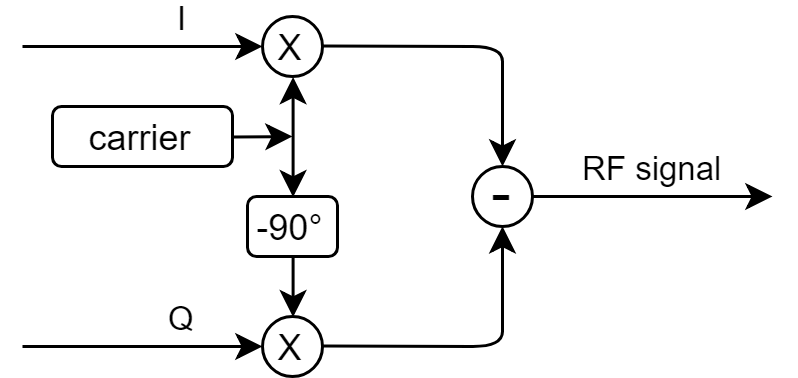
\includegraphics[width=\textwidth]{images/iqmod.png}
    		\caption{\textit{Schematic of IQ modulator}}
    		\label{fig:polarplot}
		\end{figure}
		
		\begin{figure}[!htb]
    		\centering
   			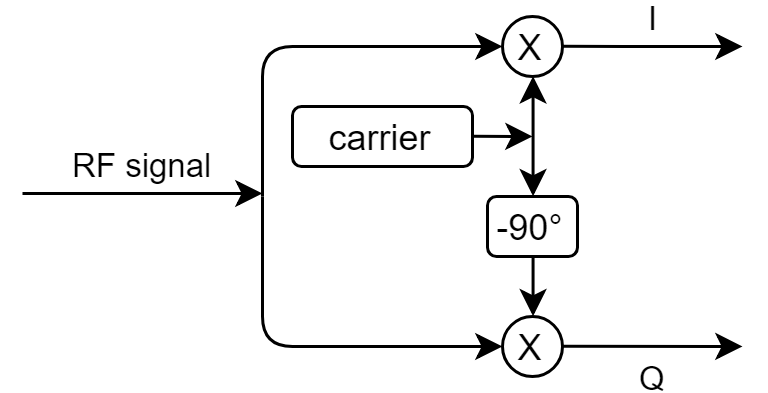
\includegraphics[width=\textwidth]{images/iqdemod.png}
    		\caption{\textit{Schematic of IQ demodulator}}
    		\label{fig:polarplot}
		\end{figure}
		\newpage
		The flexibility and simplicity of this solution compared to direct phase manipulations
		is a reason why I/Q modulators and demodulators are so widely used and popular in RF hardware.
		

	\section{IQ imbalance models}
	\section{Software Defined Radio}
		SDR (Software Defined Radio) is a radio communication system where components typically implemented in hardware 
		(e.g. mixers, filters, amplifiers, modulators/demodulators), are instead implemented by the means of software.
		
		Rapid development of technology in telecommunication field requires hardware that is able to adapt and follow these changes. 
		This need was main reason for creation of SDR systems. 
		
		
\chapter{Hardware and tools}
	This chapter describes chosen hardware, tools and explains reasons behind such decisions.
	\section{Adalm Pluto and AD tools}
		\subsection*{Adalm Pluto Board}
			Adalm Pluto is learning module from Analog Devices that can be used to introduce 
			principles of operation and theory behind SDR and RF communication.
			
			\begin{figure}[!htb]
    			\centering
   				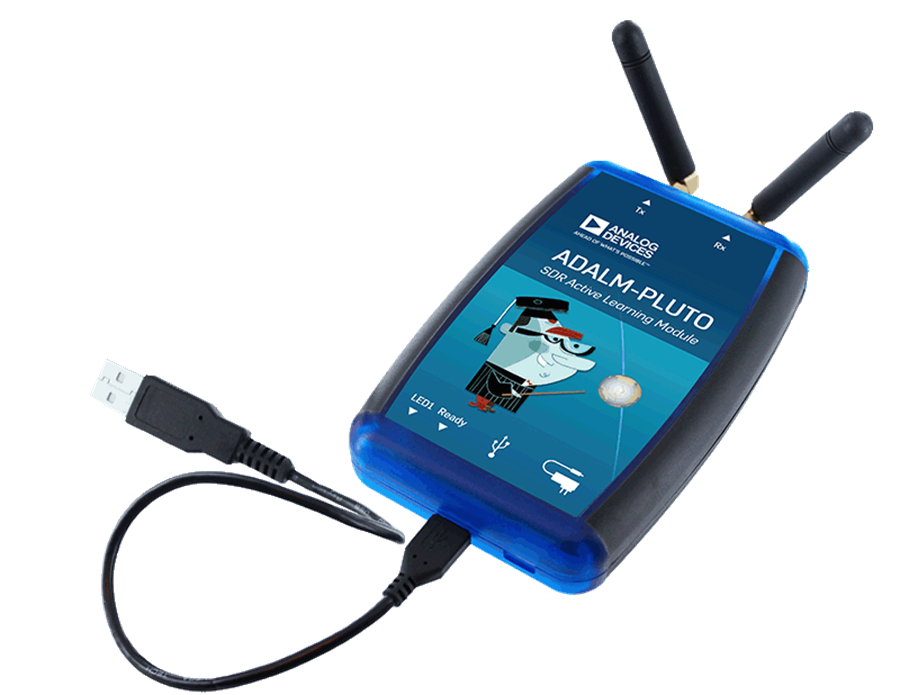
\includegraphics[width=\textwidth]{images/plutoimg.png}
    			\caption{\textit{Image of Adalm Pluto device.}}
			\end{figure}
			\newpage
			\begin{figure}[!htb]
    			\centering
   				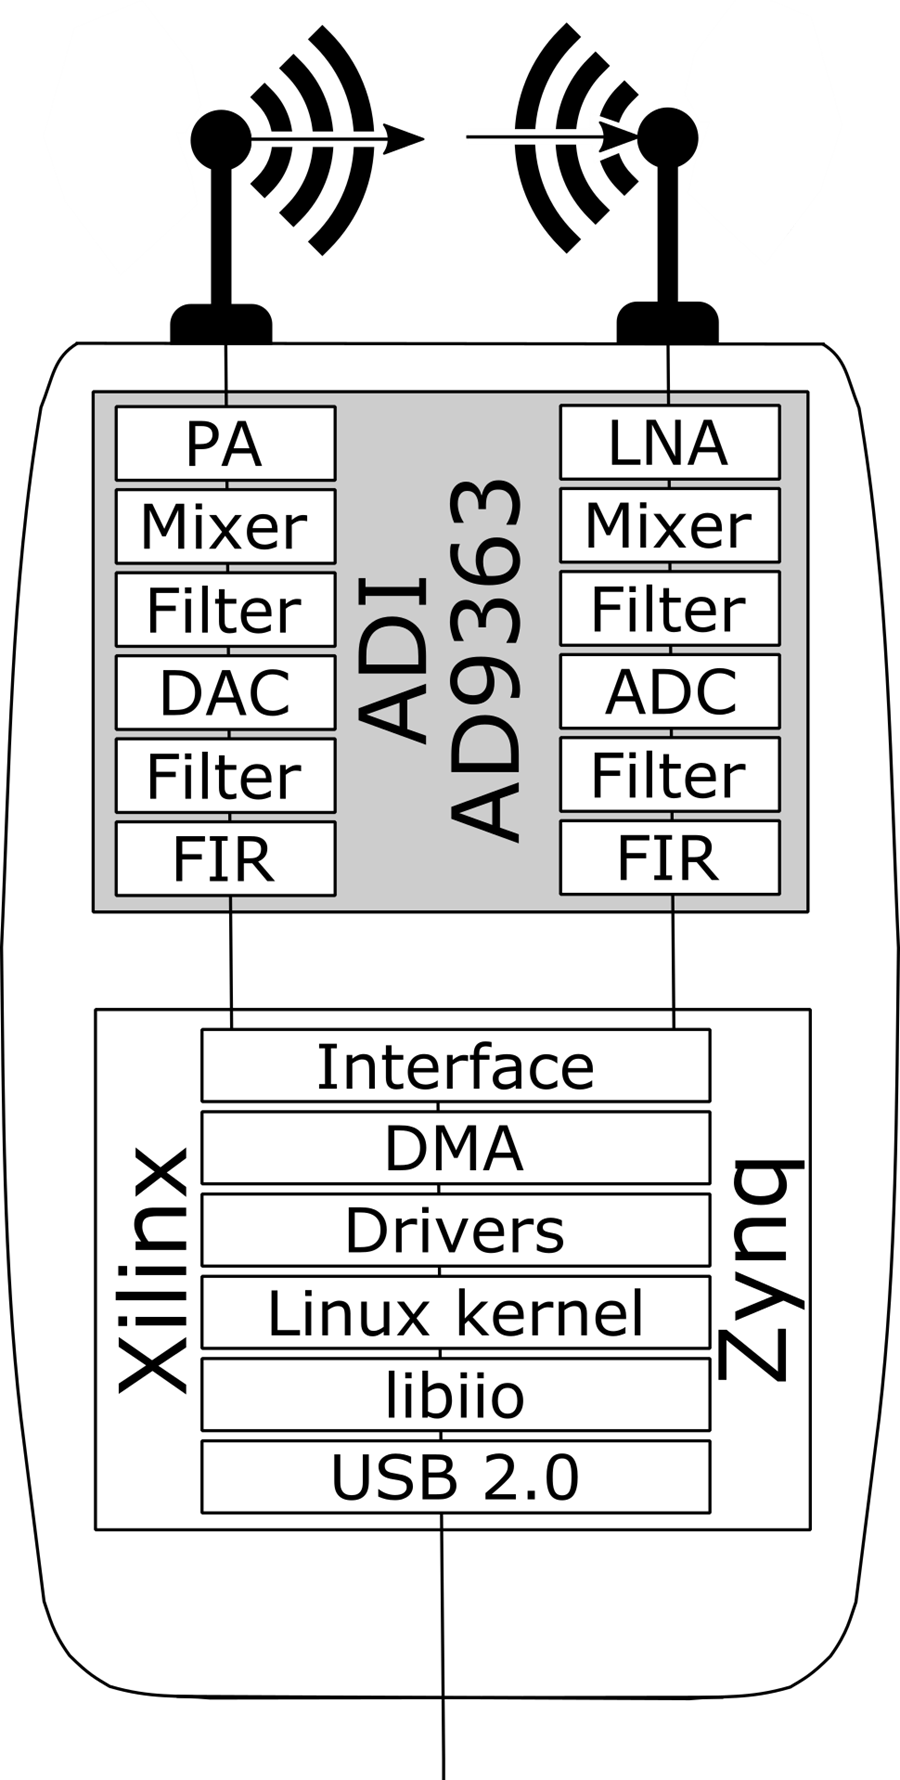
\includegraphics[width=11cm]{images/pluto_schematic.png}
   		 		\caption{\textit{Schematic Adalm Pluto hardware}}
			\end{figure}
			
			Adalm Pluto is already integrated with with MATLAB, Simulink, GNU Radio, and libIIO
			allows to interface with the devices using C, C++, C\# or Python programming languages.
			PlutoSDR is open software repository with all software and tools related to Adalm Pluto
			including: HDL Project in Xillinx Vivado, Buildroot configuration for embedded Linux.
			Main reason for choosing this SDR device was relatively low price in comparative to other
			available solutions on the market. All other devices were FPGA based. Adalm Pluto core is 			Zynq7010 SoC which is combination of ARM based processor capable of running Linux and
			FPGA part which can communicate with the processor via AXI interface.
		\subsection*{AD9363 Agile RF Transceiver}
			The main part of Adalm Pluto SDR is AD9363.  AD9363 is a high performance, highly
			integrated RF agile transceiver designed for use in 3G and 4G femtocell applications.
			
			\begin{figure}[!htb]
    			\centering
   				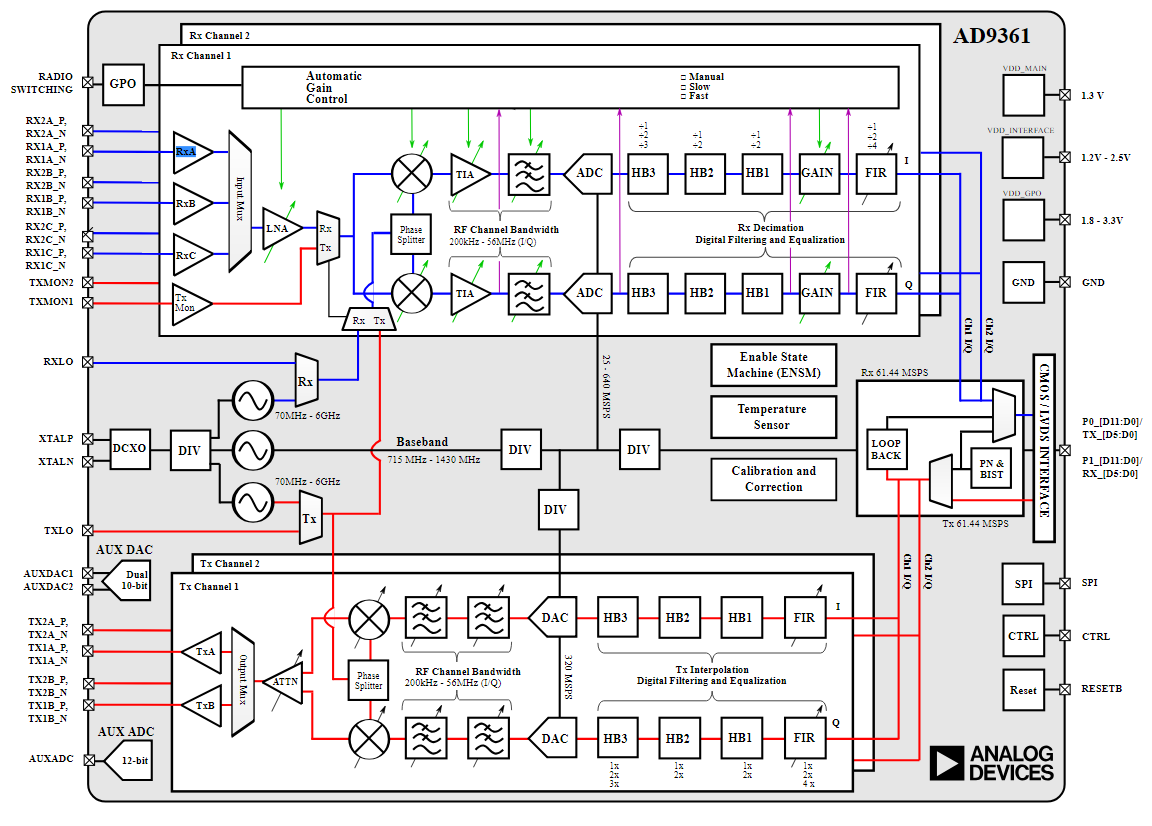
\includegraphics[width=\textwidth]{images/ad9361_sch.png}
   		 		\caption{\textit{Block diagram of AD9363 RF transceiver}}
			\end{figure}
			
			Ad9363 features:
			\begin{itemize}
				\item Wide bandwidth from 325Mhz to 3.8GHz,
				\item Tunnable channel bandwidth up to 20MHz,
				\item Independent AGC (Automatic Gain Control),
				\item Full duplex communication,
				\item DC offset and I/Q mismatch tracking.
				\item Flexible rate, 12-bit ADC and DAC
			\end{itemize}
		\subsection{IIO Osciloscope}
			The ADI IIO Oscilloscope is application which allows interfacing with different
			evaluation or custom made board based on AD agile RF Transrecivers. This program allows
			communication with the device connected with PC
			using:
			\begin{itemize}
				\item Local or remote network,
				\item USB 2.0 interface,
				\item Serial Port.
			\end{itemize}			 
			
			Application supports full configuration of the device including: configuration receiver
			frequency and channel bandwidth. Access to DC offset tracking, I/Q correction,
			internal calibration functionality and all registers. Moreover allows to process revived
			using filters designed in matlab and four gain control modes:
			\begin{itemize}
				\item manual configuration - gain is selected by user.
				\item slow attack - gain is selected to attenuate  backgrund noise as much as
				possible,
				\item fast attack
				\item hybrid attack.
				
			\end{itemize}
			\vspace{5mm}
							
			\noindent
			Program allows to plot received data from selected channels in four different modes:
			\begin{itemize}
				\item time domain as I and Q signals,
				\item frequency domain with configurable FFT and averaging size,
				\item constellation as relation between I and Q signals,
				\item cross-correlation for multi-channel boards.
			\end{itemize}

	\section{Zynq and Xilinx tools}
		\subsection*{Introduction to SoC}
		SoC is aberration from System on Chip. Such devices aggregates
		many types of hardware in single chips including: ADCs, DACs, internal memory, external 
		memory controllers, peripheral interfaces such as SPI, UART, I2C
		interfaces controllers and many others. The main idea is that single silicon chip may be
		used to implement functionality of entire system. This is cheaper and faster solution than
		realizing such functionality on PCB using separate components. In the past such role
		belonged to ASIC.
		(Application Specific Integrated Circuits). The major disadvantages of such solution is lack
		of flexibility and significant development cost and time. This makes ASIC's sustainable only
		on the high volume market where no future upgrade will be required. These limitations created
		clear need for more flexible device with faster development time. This need has been long
		satisfied by a FPGAs. FPGA can be reconfigured as desired which means virtually no risk in
		deploying solution which may require upgrade based on FPGA. Next step are SoC based solution.
		SoC is combination of processor and FPGA. This allows to create fast application dependent
		hardware functionality. Moreover processor can run normal operating system which allows fast
		development and flexibility of the solution.
		
		\subsection*{Zynq-7000 family SoC}
		The Zynq is new kind of SoC from Xillinx. It combines both applications processor and FPGA 	
		fabric. The Zynq device comprises two sections: PS (Processing System) and PL (Programmable
		Logic). This sections can be used separately for independent task or together to utilize
		advantages of both software and hardware. The Zynq devices are meant to use structure of
		both sections and interface between them. Connection between these parts is provided by AXI
		(Advanced eXtensible Interface) which is registered under ARM trademark.
		\\
		
		Processing System in all Zynq devices has the same architecture, and the base of it is
		a dual-core ARM Cortex-A9 processor. This is a hard processor which means it is manufactured 	        directly in silicon structure. Zynq allows to use soft processors like PicoBlaze and 
		MicroBlaze which can be implemented in PL sections. Depending on the size and speedgrade of
		the device ARM processor is accompanied by set of processing resources e.g (MMU, DMA, SRAM,
		Processing System External Interfaces, cache memory, control registers , etc.) which forms
		together APU (Application Processing Unit).
		
		\begin{figure}[!htb]
    		\centering
   			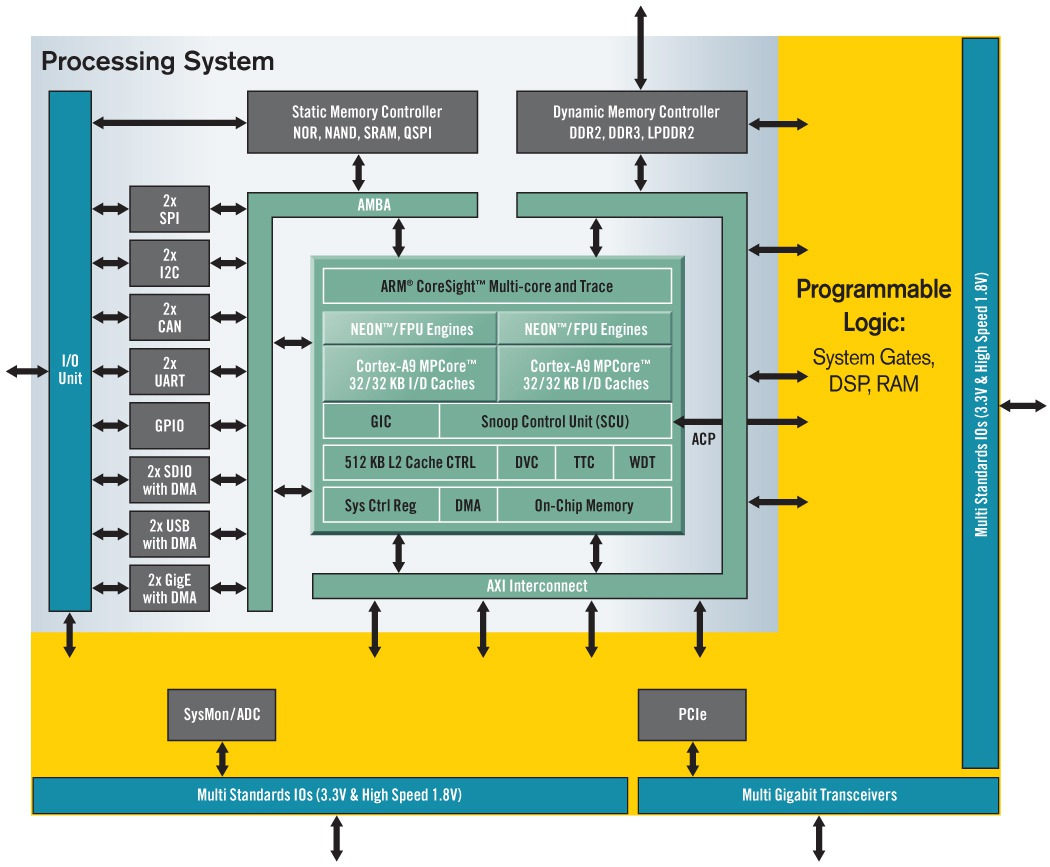
\includegraphics[width=\textwidth]{images/zynq.jpeg}
   		 	\caption{\textit{Block diagram fo Zynq 7000 family SoC}}
		\end{figure}
		\newpage

		Programmable Logic is a FPGA based on Atrix-7 and Kintex-7 fabric from Xillinx. PL consist of
		CLBs ( Configurable Logic Blocks ), slices, IOBs( Input Output Blocks), LUTs (Lookup tables),
		fliplops and switch matrices. Additionally there are BRAM (Block Random Access Memory) which
		are used to store large amout of date in small part of the device which allows fast access to
		its content. Second additional resource is DSP48E1 slice. This is advanced DSP module that
		allows many complex mathematical operation in a single clock cycle.
		
		

	\section{Simulation environment}
	
\chapter{Algorithms}
	This chapter describes all algorithms used for signal quality improvement. All of considered 
	algorithms are blind. This means that signal analysis is purely statistical with no prior 
	information about signal. Advantages of this approach is that this algorithms can be used 
	for any type of possible signal.
	\section{DC offset correction}
		This section describes algorithms used for removing DC offset from revived samples.
		\subsection*{Moving Average Filter}
			Moving Average Filter is simple FIR (Finite Impulse Response) filter. This filter is
			commonly used for white noise removal and signal smoothing. However when filter order
			is great enough to account for samples from full period of the signal filters the
			average represents signal DC offset.
			
			The filter equations is presented below:
			\[
				y[n] = \frac{1}{N} \sum_{k=0}^{N-1}x[n-k],
			\]
			where:
			\begin{itemize}
				\item   $N$ is order of the filter.
				\item	$y[n]$ is filtered sample at n-th step,
				\item   $x[n]$ is n-th sample from receiver.
			\end{itemize}
			Corrected values are calculated as follows:
			\[
				I/Q_{corr} = I/Q - I/Q_{mean},
			\]
			where:
			\begin{itemize}
				\item I/Q is recived I/Q sample,
				\item $I/Q_{mean}$ is DC offset calculated using Moving Average Filter.
			\end{itemize}

			Algorithm introduces delay by N samples in the signal. 
		\subsection*{Normalized Gaussian Filter}
			Normalized Gaussian Filter is filter whose impulse response has shape of Gaussian
			function with all values in range from 0 to 1.
			
			\[
				G(x) = \frac{1}{ \sqrt{2\pi \sigma^2}}e^{\frac{-x}{2\sigma^2}}
			\]
			where:
			\begin{itemize}
				\item $x$ is 
				\item $\sigma$ is standard deviation. 
			\end{itemize}
			
			The filter equations is presented below:
			\[
				y[n] = \sum_{k=0}^{N-1}x[n-k]G(x)
			\]
			\begin{itemize}
				\item N is windows size,
			\end{itemize}			
			Corrected values are calculated as follows:
			\[
				I/Q_{corr} = I/Q - I/Q_{gauss},
			\]
						where:
			\begin{itemize}
				\item I/Q is recived I/Q sample,
				\item $I/Q_{gauss}$ is DC offset calculated using Normalized Gauss Filter.
			\end{itemize}
			This filter has better performance in frequency domain than Moving Average Filter.
	\section{Magnitude and Phase Correction}
		The I/Q imbalance is common problem in RF front-ends that uses analog quadrature down-
		mixing. The ideal down-converter performs only simple frequency shift. Real down-
	    converters introduces image interference which may be assumed as constant. But amplifiers
	    and filters introduces varying with frequency imbalance.
	    
	    In ideal case the receiver output is:
		\begin{equation}
			\renewcommand*{\arraystretch}{1.3} 
			\begin{array}{ll}
				I(t) = cos(\omega t) \\
				Q(t) = sin(\omega t) \\
			\end{array}
		\end{equation}
		where:
		\begin{itemize}
			\item $\omega$ is tone frequency.
		\end{itemize}
	    I and Q components are orthogonal with respect to each other.
	    
	    In real case, assuming Single Branch Model receiver output is:
		\begin{equation}
			\renewcommand*{\arraystretch}{1.3} 
			\begin{array}{ll}
				I(t)' = \alpha cos(\omega t) + \beta_I \\
				Q(t)' = sin(\omega t + \phi) + \beta_Q \\
			\end{array}
		\end{equation}
		where:
		\begin{itemize}
			\item $\alpha$ is magnitude mismatch,
			\item $\phi$ is phase imbalance,
			\item $\beta_{I/Q}$ is signal DC offset.
		\end{itemize}
		Input of phase correction algorithms is signal with DC offset extracted using algortihms
		from previews section. Hence the signal model is:
		\begin{equation}
			\renewcommand*{\arraystretch}{1.3} 
			\begin{array}{ll}
				I(t)'' = \alpha cos(\omega t) \\
				Q(t)'' = sin(\omega t + \phi) \\
			\end{array} \label{eq:iqreal}
		\end{equation}
		According to Ptolemy’s identitie for the sine of sum:
		\[
			sin\left(\omega t + phi\right) = 
			sin\left(\omega t\right))cos\left(\phi \right) + 
			cos\left(\omega t\right) sin\left(\phi \right)
		\] 
		Equation \ref{iq:real} be rewritten in matrix form as:
		\begin{equation}
			\begin{bmatrix}
				I(t)'' \\
				Q(t)''
			\end{bmatrix}
			=
			\begin{bmatrix}
				\alpha & 0 \\
				sin(\phi) & cos(\phi)
			\end{bmatrix}
			\begin{bmatrix}
				I(t) \\
				Q(t)
			\end{bmatrix} \label{eq:iqrealmat}
		\end{equation}
		After multiplying both sides of \ref{eq:iqrelamat} by inversion of parameters matrix following set of exuations
		is obtained:
		\begin{equation}
			\begin{bmatrix}
				I(t) \\
				Q(t)
			\end{bmatrix}
			=
			\begin{bmatrix}
				\alpha^{-1} & 0 \\
				\alpha^{-1}tan(\phi) & sec(\phi)
			\end{bmatrix}
			\begin{bmatrix}
				I''(t) \\
				Q''(t)
			\end{bmatrix}
		\end{equation}
		This shows that only $\alpha$ and $\phi$ must be found to perform I/Q mismatch
		compensation. According to this paper:
		\[
			<I''(t)I''(t)> = \frac{1}{2}\alpha^2
		\]
		\[
			\alpha = \sqrt{2<I''(t)I''(t)>}
		\]
		\[
			<I''(t)Q''(t)> = \frac{1}{2}\alpha^2sin(\phi)
		\]
		\[
			sin(\phi)= \frac{2}{\alpha}<I''(t)Q''(t)>
		\]
		Assuming that $|\phi| \leq \frac{pi}{4}$ $cos(\phi)$ can be obtained directly from
		$\sin(\phi)$ using following formula:
		\[
		 	cos(\phi) = \sqrt{1-sin(\phi)}
		\]
		Using following parameters in we can substitute matrix equations \ref{eq:iqrealmat} with:
		\begin{equation}
			\begin{bmatrix} 
				I(t) \\
				Q(t)
			\end{bmatrix}
			=
			\begin{bmatrix}
				\frac{1}{\alpha} & 0 \\
				\frac{-sin(\phi)}{acos(\phi)} & \frac{1}{cos(\phi)}
			\end{bmatrix}
			\begin{bmatrix}
				I''(t) \\
				Q''(t)
			\end{bmatrix}\label{eq:iqcorr}
		\end{equation}
		The I/Q mismatch correction  can be now applied using \ref{eq:iqcorr} formula.
\chapter{Simulations}
Chapter with all algorithms simulation in Matlab.
	\section{Single tone signal}
	\section{Multitone signal}
	\section{QAM modulation}
	
\chapter{Measurements}
Chapter with all algorithms implemented in Zynq PL.
	\section{Single tone signal}
	\section{Multitone signal}
	\section{QAM modulation}


\chapter{ Conclusions}


\addcontentsline{toc}{chapter}{Bibliography} %utworzenie w spisie treści pozycji Bibliografia
\bibliography{bibliografia} % wstawia bibliografię korzystając z pliku bibliografia.bib - dotyczy BibTeXa, jeżeli nie korzystamy z BibTeXa należy użyć otoczenia thebibliography

\begin{thebibliography}{9}
\bibitem{highSpeedDesign} 
Stephen H. Hal, Garrett W. Hall, and James A. McCall. 
\textit{High-Speed Digital System Design - A Handbook of Interconnects Theory and Design Practices}.
New York, Chichester, Weinheim, Brisbane, Singapore, Toronto, 2000.


\end{thebibliography}
%opcjonalnie może się tu pojawić spis rysunków i tabel
% \listoffigures
% \listoftables
\end{document}
